\documentclass[12pt]{article}
\usepackage{amssymb,amsmath,
latexsym, amsthm}
\usepackage{mathtools}
\usepackage{mathrsfs}
\usepackage[english]{babel}
\usepackage[utf8]{inputenc}
\usepackage{fancyhdr}
\usepackage{titlesec} % Decrease 
  % spacing after titles

\usepackage{sectsty}

\usepackage{url}
\usepackage{graphicx}
\usepackage{xcolor}

\newcommand{\N}{\mathbb{N}}
\newcommand{\Z}{\mathbb{Z}}
\newcommand{\Q}{\mathbb{Q}}
\newcommand{\R}{\mathbb{R}}
\newcommand{\C}{\mathbb{C}}
\newcommand{\PP}{\mathbb{P}}
\newcommand{\D}{\mathbb{D}}

\newcommand{\LL}{\mathcal{L}}
\newcommand{\BB}{\mathcal{B}}
\newcommand{\AAA}{\mathcal{A}}
\newcommand{\ff}{\mathcal{F}}
\newcommand{\pp}{\mathcal{P}}
\newcommand{\M}{\mathcal{M}}

\newcommand{\HH}{\mathscr{H}}

\newcommand{\tr}{\text{tr}}
\newcommand{\rank}{\text{rk}}
\newcommand{\en}{\text{End}}
\newcommand{\aut}{\text{Aut}}
\newcommand{\Hom}{\text{Hom}}
\newcommand{\nul}{\text{null}}
\newcommand{\im}{\text{im}}

\titlespacing\section{0pt}{0pt plus 4pt minus 2pt}{-5pt plus 2pt minus 2pt}
\titlespacing\subsection{10pt}{0pt plus 4pt minus 2pt}{0pt plus 2pt minus 2pt}
\titlespacing\subsubsection{10pt}{0pt plus 4pt minus 2pt}{0pt plus 2pt minus 2pt}



\newcommand{\sinti}{\,\,\mathrel{\int\!\!\!\!\!\!\!\sim}_{\mathclap{I}}} 
% Intergral with squiggle thru it



\newcommand\invisiblesubsection[1]{%
  \refstepcounter{subsection}%
  \addcontentsline{toc}{subsection}{\protect\numberline{\thesubsection}#1}%
  \subsectionmark{#1}}



\setlength{\oddsidemargin}{-0,25in} % Left margin of 1 in + 0 in = 1 in
\setlength{\textwidth}{7in}   % Right margin of 8.5 in - 1 in - 6.5 in = 1 in
\setlength{\topmargin}{-.5in}  % Top margin of 2 in -0.75 in = 1 in
\setlength{\textheight}{9.2in}  % Lower margin of 11 in - 9 in - 1 in = 1 in
\setlength\parindent{0pt}

\renewcommand{\baselinestretch}{1.5}

%%%%%%%%%%%%%%%%%%%%%%%%%%%%%%%%%%%%


\theoremstyle{plain}
\newtheorem{thm}{Theorem}[section]
\newtheorem{lem}[thm]{Lemma}
\newtheorem{prop}[thm]{Proposition}
\newtheorem*{cor}{Corollary}

\theoremstyle{definition}
\newtheorem{defn}{Definition}[section]
\newtheorem{conj}{Conjecture}[section]
\newtheorem{exmp}{Example}[section]



%%%%%%%%%%%%%%%%%%%%%%%%%%%%%%%%%%


\pagestyle{fancy}
\fancyhf{ }
\lhead{Robot Vision - Fall 2019}
\rhead{Dr. Niels da Vitoria Lobo}



\begin{document}

\begin{center}
\begin{Large} 
MNIST Assignment\\
\end{Large}
\end{center}

In this assignment, you will implement Python code to perform classification on the MNIST dataset using the deep learning framework Keras. There are two parts to the assignment. The \textit{first} is to run the experiment with the instructions below, copy those results to a text file, and submit them to the instructor-specified location/grader. The \textit{second} part of the assignment will be to run your code in the presence of a grader to confirm it runs as expected. In order to receive full credit, please follow the instructions below exactly.

\section*{Part I}
\begin{enumerate}
\item Navigate to \url{https://keras.io/examples/mnist_cnn/}. Copy and paste the code into a PyCharm project. If you choose to use a Jupyter Notebook or Google CoLab, your submitted .txt document must look the same as if you ran it in PyCharm.

\item Immediately following the line containing \textbf{\textcolor{blue}{epochs = 12}}, add the line 
\vspace{-4mm}
\begin{center}
\textbf{\textcolor{blue}{np.random.seed(0)}}
\end{center}
\vspace{-4mm}
Keras gets its source of randomness from numpy's random number generator. To ensure reproducible results, this starts random computation off
at the same place every run.

\item Immediately \textbf{following} the line containing \\ \textbf{\textcolor{blue}{model.add(Dense(num\_classes, activation='softmax'))}} and \textbf{before} the line containing \textbf{\textcolor{blue}{model.compile...}}, add the line
\vspace{-4mm}
\begin{center}
 \textbf{\textcolor{blue}{print(model.summary())}}
 \end{center} 
\vspace{-4mm} 
This will print a summary of your model's architecture and parameters.

\item Change the line that has \textbf{\textcolor{blue}{model.fit(...}} to 
\vspace{-4mm}
\begin{center}
\textbf{\textcolor{blue}{history = model.fit(...}}
 \end{center} 
\vspace{-4mm}

\item Delete the last three lines of code, i.e.  \textbf{\textcolor{blue}{score = ...}},  \textbf{\textcolor{blue}{print('Test...}}, and  \textbf{\textcolor{blue}{print('Test...}} and replace them with 
\vspace{-4mm}
\begin{center}
\textbf{\textcolor{blue}{print([(key, round(value[0], 4)) for key, value in history.history.items()])}}
\end{center}
\vspace{-4mm}

\item In PyCharm, we will use the ``Terminal" to run our code. The \textbf{only} reason for this is so that the output is easier for the grader to read. As shown in \textbf{Figure 1} below, go to the bottom of the PyCharm window and click ``Terminal".

\begin{center}
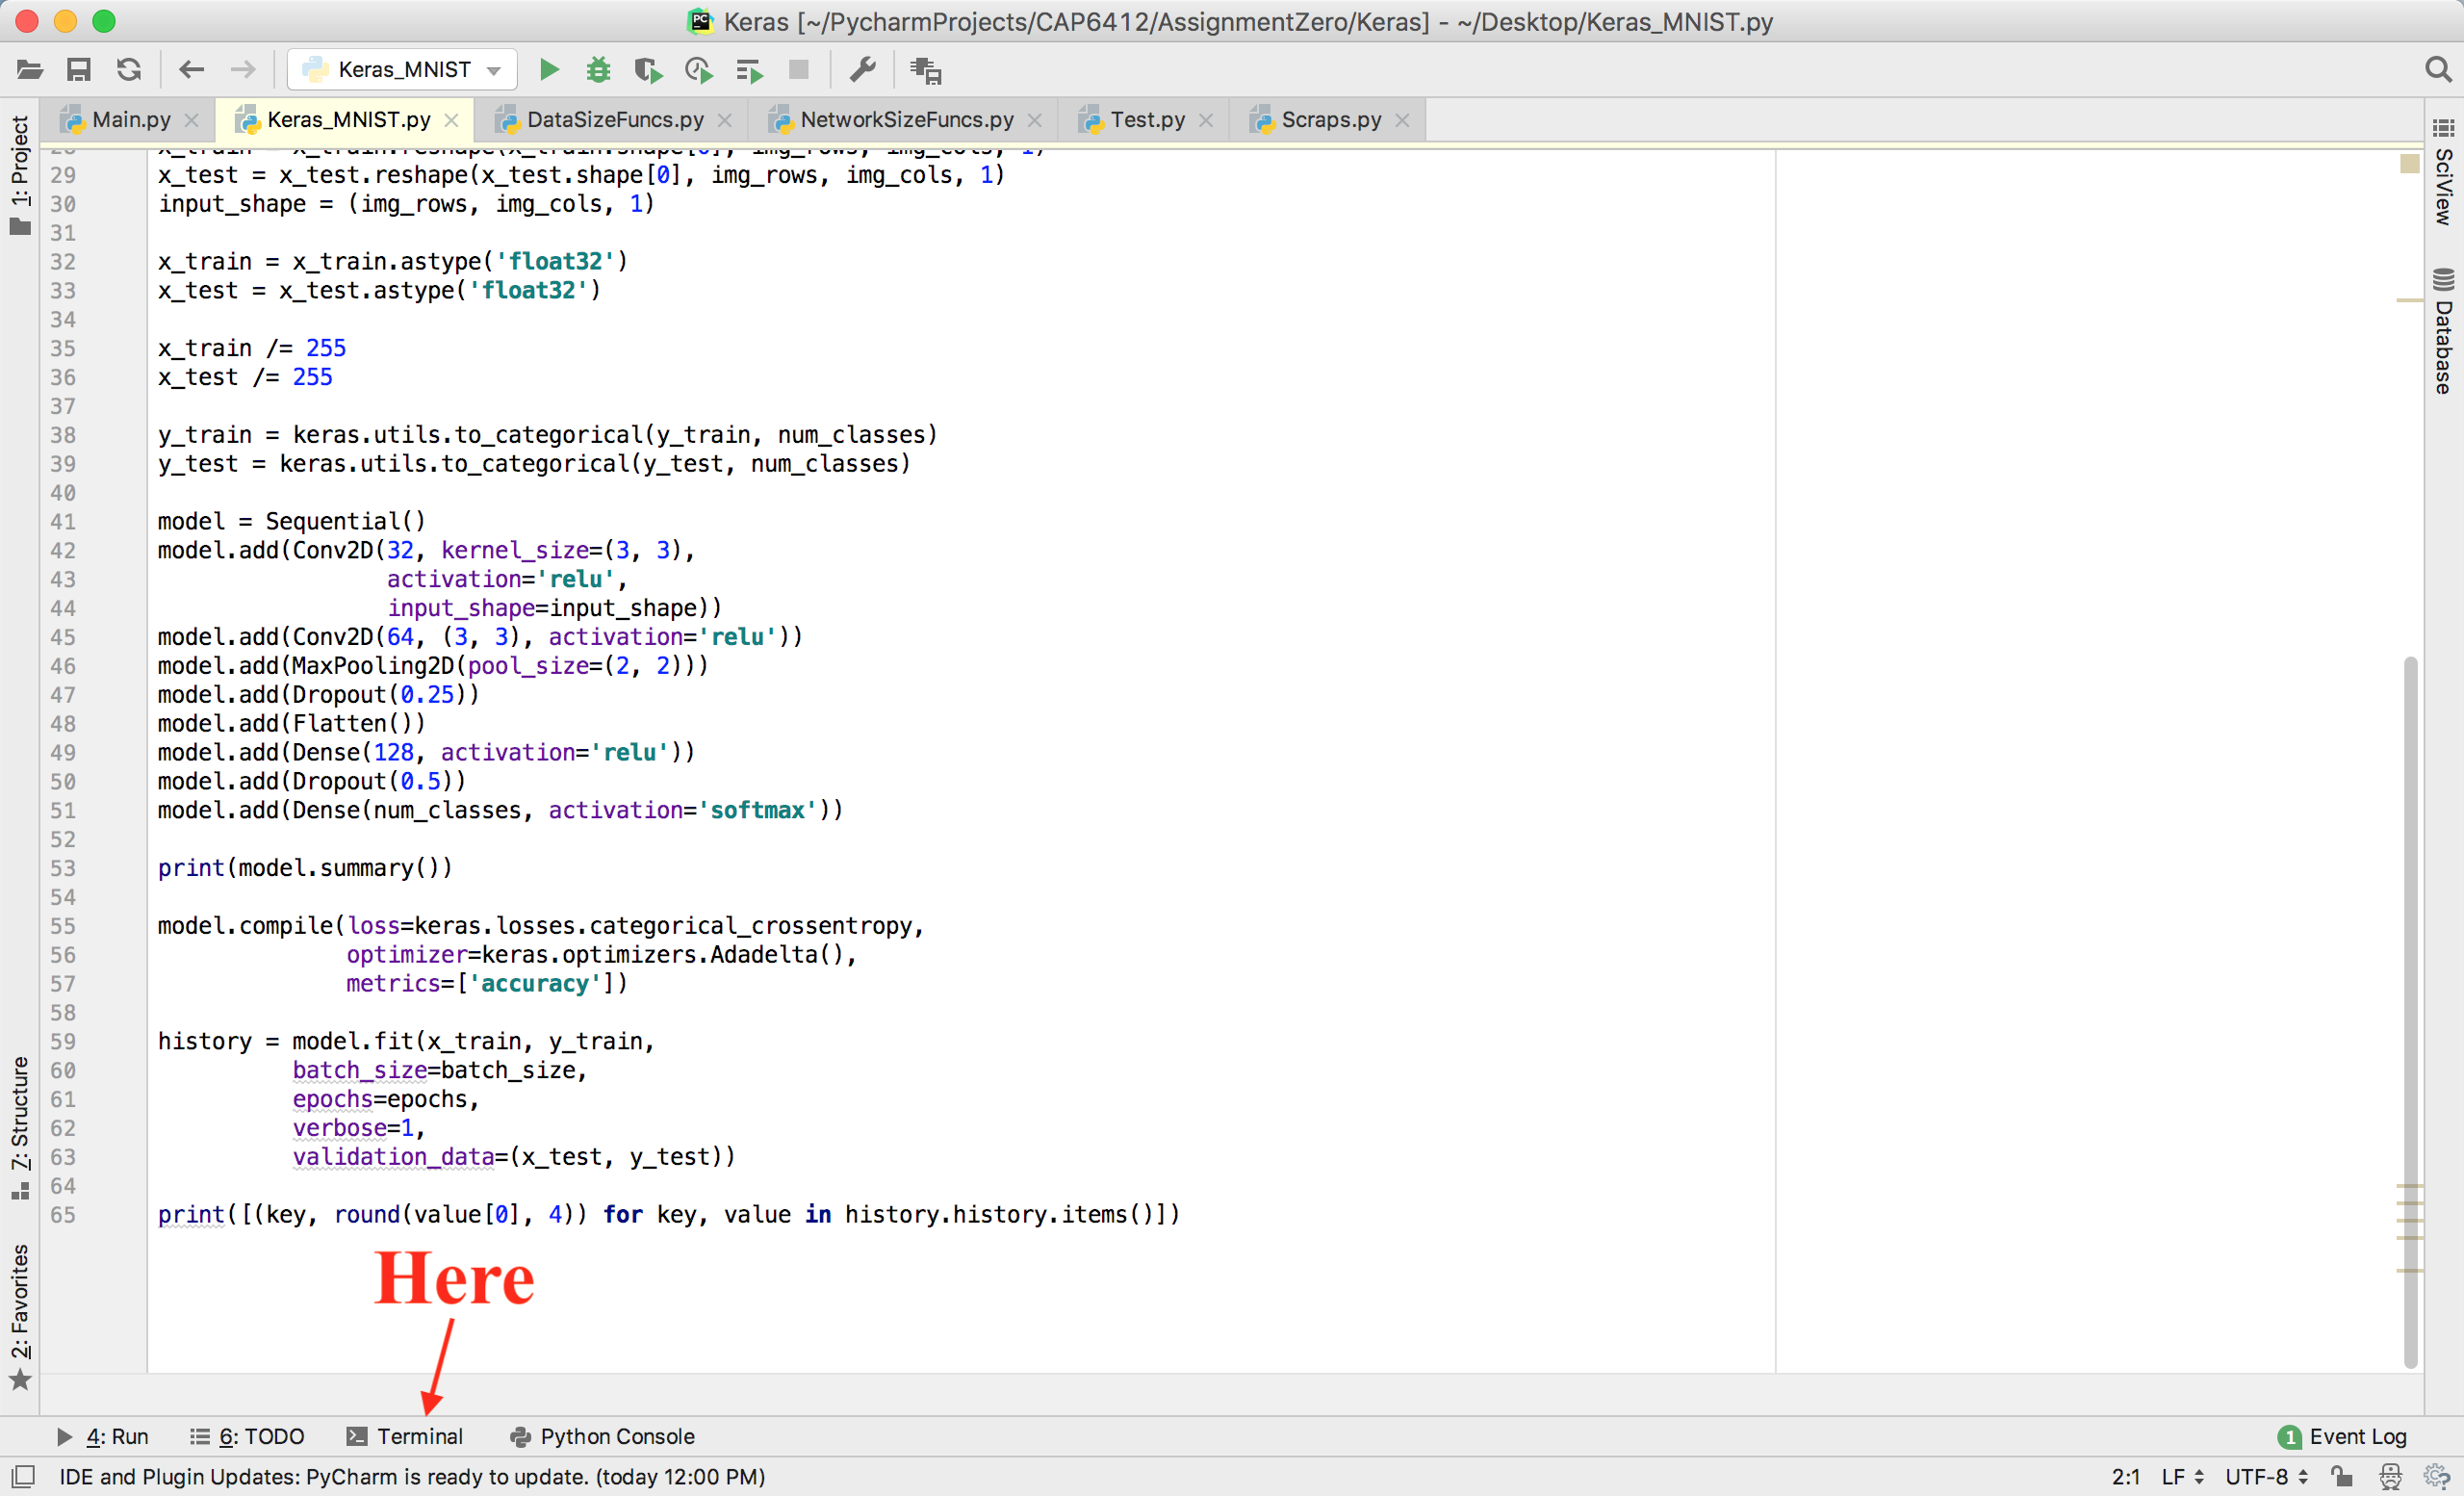
\includegraphics[scale=.25]{run1}\\
\textbf{Figure 1: Open Terminal in PyCharm.}
\end{center}

\item In the Terminal window (see \textbf{Figure 2}), activate your anaconda environment by typing
\vspace{-4mm}
\begin{center}
\textbf{\textcolor{blue}{source activate your\_env\_name}} (Mac/Linux)\\
or\\
\textbf{\textcolor{blue}{activate your\_env\_name}} (Windows)\\
 \end{center} 
\vspace{-4mm}

\item Run your code in the Terminal by typing
\vspace{-4mm}
\begin{center}
\textbf{\textcolor{blue}{python your\_code\_name.py}}
 \end{center} 


\begin{center}
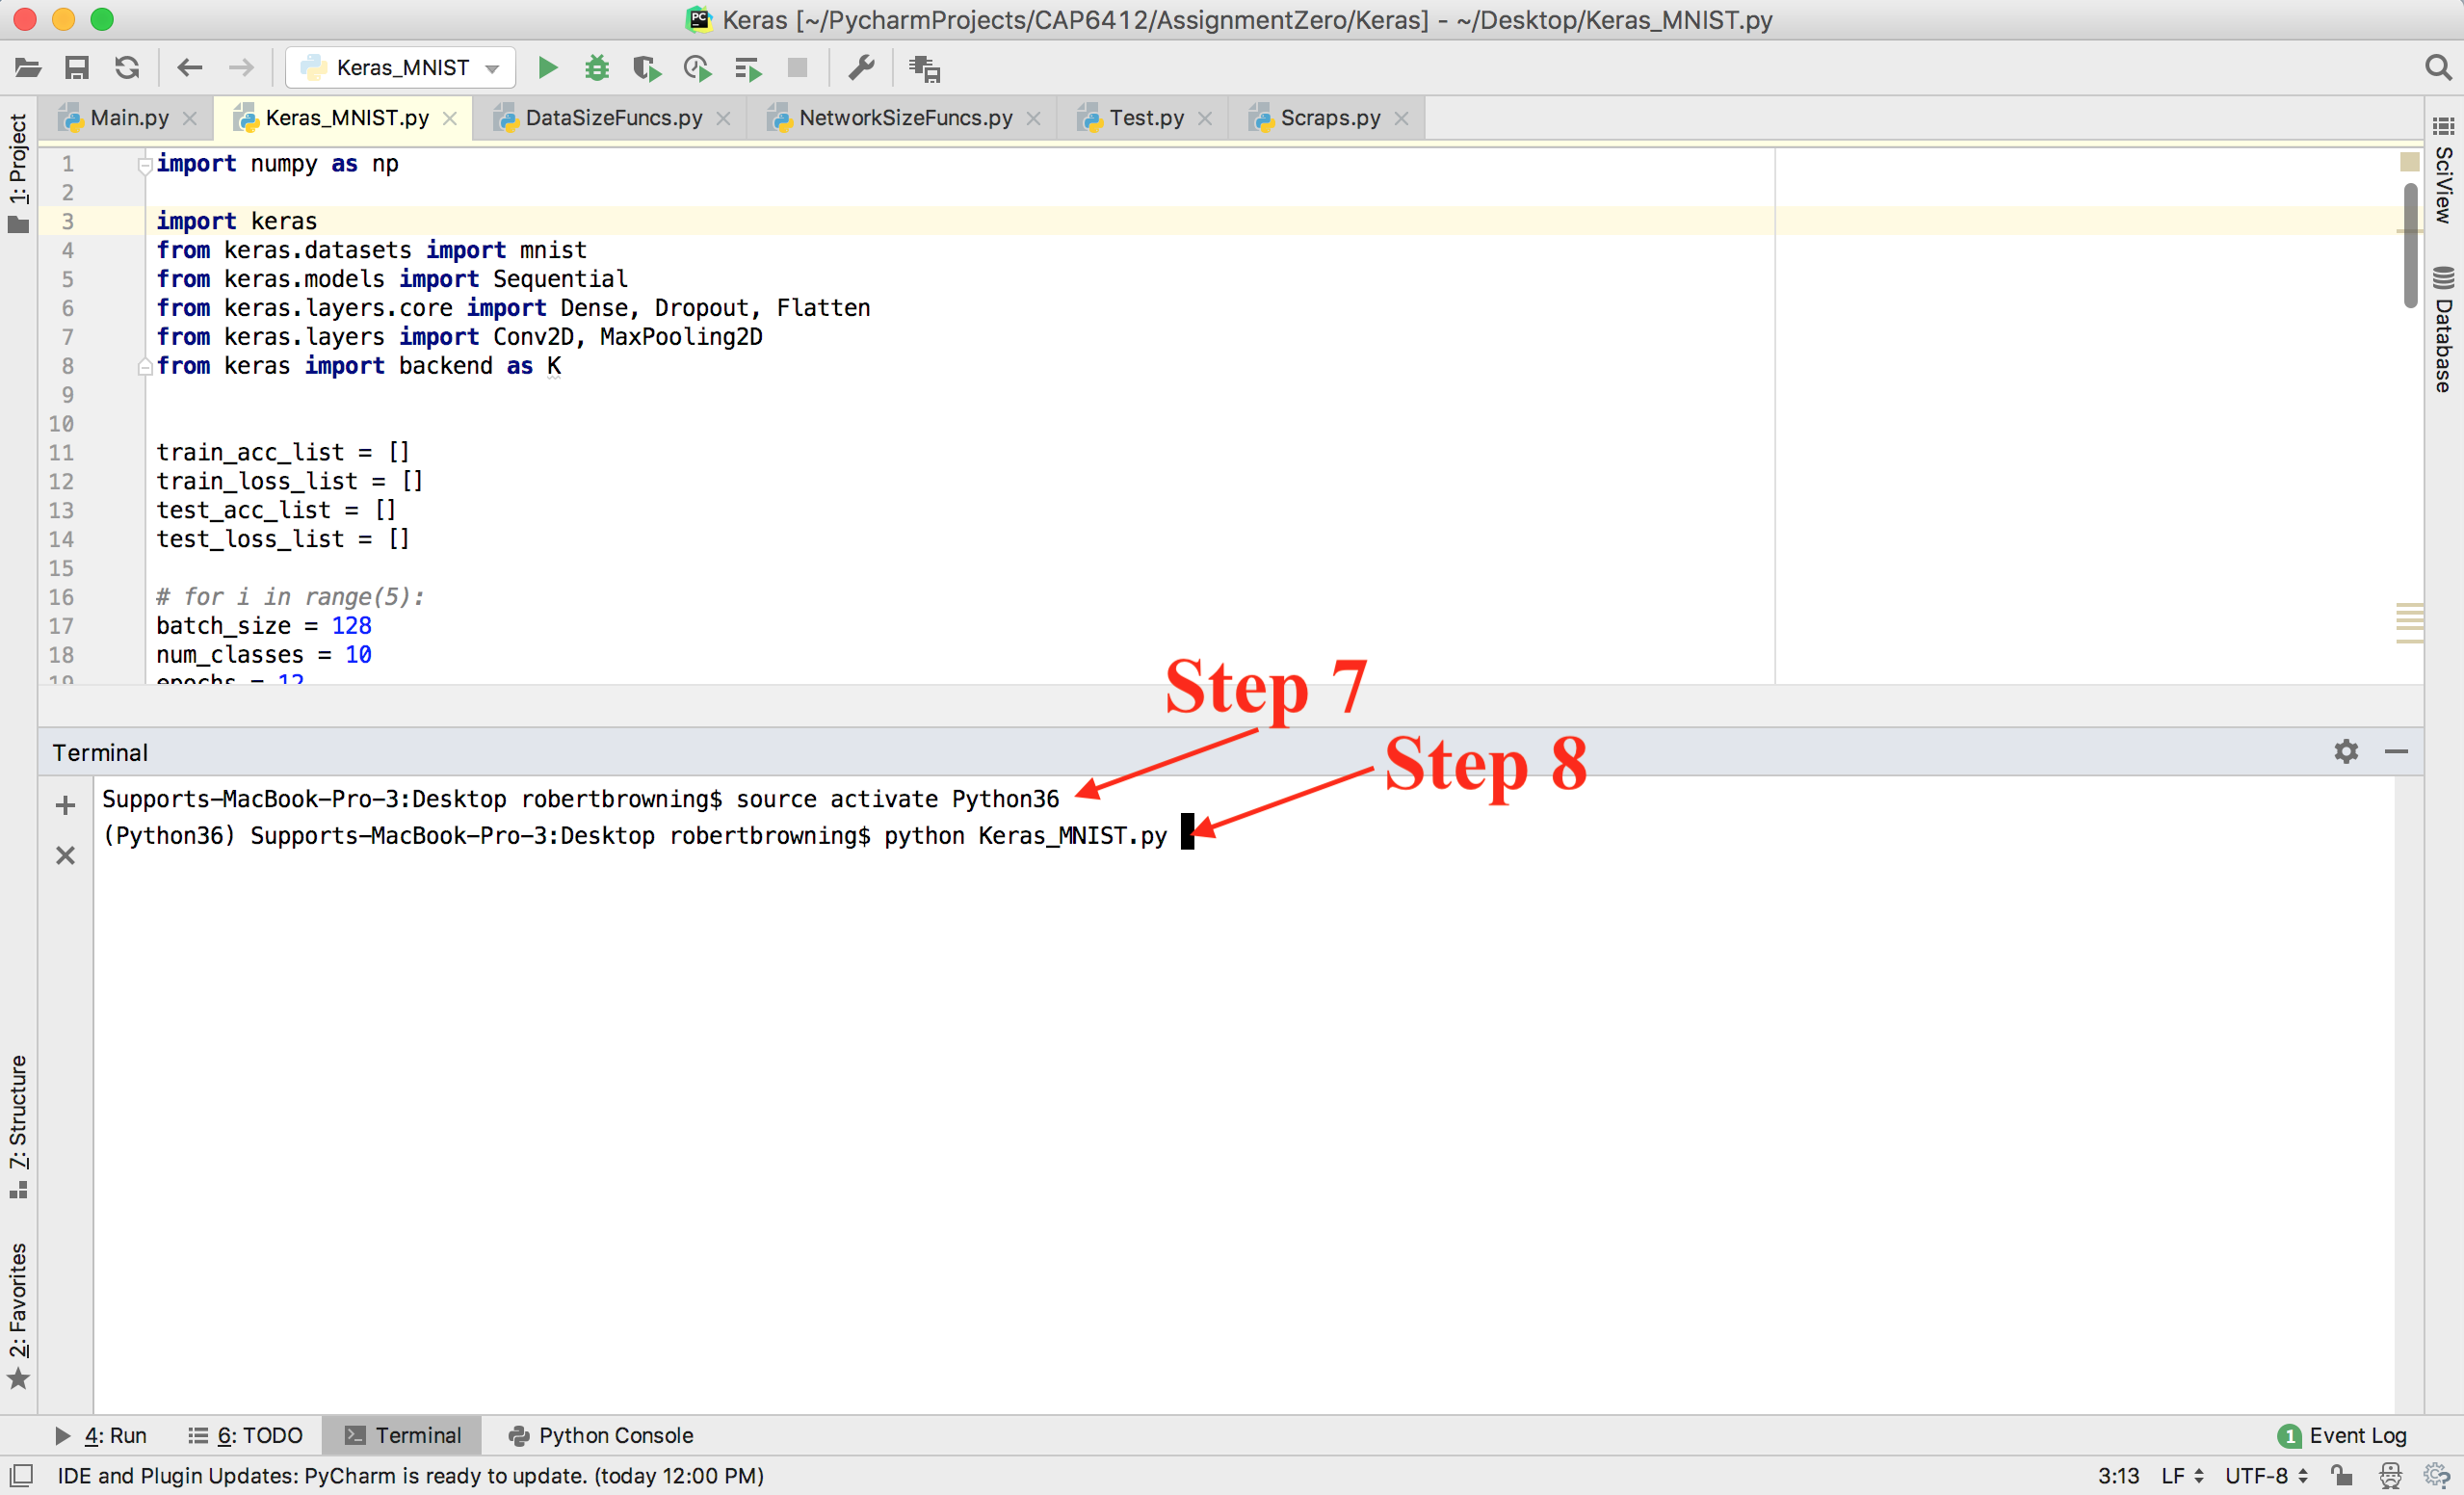
\includegraphics[scale=.25]{run2}\\
\textbf{Figure 2: Activate Environment and Run Code in Terminal.}
\end{center}

\item Finally, copy and paste your Terminal window output to a text file, FirstLastName\_MNIST.txt. Their may be some TensorFlow warnings at the start of your code. If your code continues to run correctly after those appear, simply disregard them.

To recap, your output should have, in this order 
\begin{enumerate}
\item[(i)] Your model summary,
\item[(ii)] 12 progress bars, one for each epoch
\item[(iii)] A list with four tuples, e.g. ``[('val\_loss', 1.8283), ('val\_acc', 0.436), ('loss', 1.9965), ('acc', 0.331)]"
\end{enumerate}

\end{enumerate}

\section*{Part II}

For this part of the assignment, you will exhibit to the grader that your code is working properly.
\begin{enumerate}
\item In the same code you built in \textbf{Part I}, change the number of epochs to 1, i.e. \textbf{\textcolor{blue}{epochs = 1}}.

\item Immediately following the line containing \\ \textbf{\textcolor{blue}{(x\_train, y\_train), (x\_test, y\_test) = mnist.load\_data()}}, add the following four lines:
\begin{center}
\begin{tabular}{l}
\textbf{\textcolor{blue}{x\_train = x\_train[0:1000] }} \\
\textbf{\textcolor{blue}{y\_train = y\_train[0:1000] }} \\
\textbf{\textcolor{blue}{x\_test = x\_test[0:1000] }} \\
\textbf{\textcolor{blue}{y\_test = y\_test[0:1000]  }} 
\end{tabular}
\end{center}

This will reduce the size of your dataset considerably so your code will run much faster.

\item Run the code for the grader to see. You can run this one in \textit{either} PyCharm console or the terminal window. Jupyter and CoLab users will need to re-run all cells. 
\end{enumerate}

\end{document}
